\chapter{Analyse de domaine}\label{chap:domain}
\begin{preamble}
Le chapitre précédent nous donne une fondation solide pour déployer des services contextuels dans une maison connectée, 
en assurant la fiabilité de son infrastructure de capteurs. 
Nous pouvons désormais nous intéresser au développement de ces services contextuels.
Pour cela, nous allons analyser dans ce chapitre un large éventail de services d'assistance domiciliaire 
dédiés aux personnes âgées, en considérant la variété des besoins des 
intervenants. 
%Ces services sont installés sur la plate-forme d'assistance domiciliaire DomAssist-2 déployée chez 129 personnes 
%âgées vivant seules et âgées de 82 ans en moyenne~\paulcite{consel2017homeassist}. 
Cette analyse permet d'identifier les concepts communs et les variations
entre différentes couches de services déployés et utilisés au quotidien,
pour en extraire des concepts clés et des opérations spécifiques aux
traitements sensibles au contexte\footnotemark{}\footnotetext{Ce travail à fait l'objet d'une soumission~:~\fullcite{carteron2017domain}.}.
\end{preamble}
\chpsummary{Aperçu}
{
{\em DomAssist} Présentation d'une expérimentation écologique large échelle sur laquelle nous nous appuyons pour notre analyse.;
{\em Analyse de domaine} Identification des concepts clés, des opérations spécifiques et des besoins communs aux services sensibles au contexte.
}

Les services d'assistance dédiés au maintien à domicile
des personnes âgées sont encore un domaine émergeant et le chemin vers l'adoption
reste un sujet d'étude~\paulcite{kaye2017making}. La littérature
comporte encore peu d'articles concernant le déploiement de solutions
d'assistance dans de vrais domiciles~\paulcite{kaye2011intelligent}. 
Cependant, nous avons pu faire levier
sur le projet DomAssist pour conduire notre analyse du domaine.

\section{Enjeux d'une expérimentation écologique à large échelle}\label{domain:expe}
L'étude pilote de la plate-forme, DomAssist, présentée dans le 
Chapitre~\ref{cha:fiabilite}, a donné des résultats 
encourageants quant à l'acceptabilité de la technologie, par un groupe de 24 
utilisateurs, âgés de 80 ans en moyenne, pendant une durée 
de 9 mois. D'un point de vue technologique, cette expérimentation, était une 
première confrontation aux difficultés et contraintes d'un déploiement écologique.
Nous avons donc conçu l'approche présentée dans le Chapitre~\ref{cha:fiabilite}
pour nous assurer du bon fonctionnement de l'infrastructure de
capteurs, lors de son installation et durant son exploitation, et pour garantir la consistance des 
services d'assistance.

Faisant suite à l'étude pilote, une nouvelle expérimentation
d'autonomie domiciliaire des personnes âgées est en cours à plus large
échelle, couvrant un plus grand nombre d'utilisateurs pour une durée
de 12 mois\footnote{\url{http://phoenix.inria.fr/research-projects/homeassist-500}}. La plate-forme est actuellement déployée chez 129
personnes vivant seules et âgées de 82 ans en
moyenne~\paulcite{consel2017homeassist}.  Cette expérimentation est
construite en lien étroit avec les acteurs du domaine de l'autonomie
domiciliaire des personnes âgées. Ainsi, la conception et la mise en
place des services ont impliqué tous les acteurs~: utilisateurs,
aidants, ergothérapeutes, psychologues, experts en facteurs humains,
techniciens d'installation et de maintenance et informaticiens.  Le
modèle d'assistance qui en résulte offre des services dédiés à des
tâches variées comme les rappels de rendez-vous, la surveillance
d'activités du quotidien ainsi que leur rappel si elles ne sont pas
effectuées, la sécurisation de l'utilisateur, ou encore le bilan
quotidien des activités.  L'analyse des données recueillies permet
d'évaluer et d'adapter l'assistance en fonction de chaque utilisateur
et de ses dégradations éventuelles.

Cette étude à large échelle offre de nombreux avantages pour
construire notre analyse du domaine~: (1) elle est déployée dans des
environnements réels~; (2) elle constitue un soutien pour le maintien
à domicile de personnes âgées avec des utilisateurs fragiles ayant des
besoins immédiats. La précédente expérimentation avait pour but
principal d'ajuster et de valider la plate-forme DomAssist en tant que
plate-forme d'assistance domiciliaire, en n'incluant pas
d'utilisateurs avec un statut fonctionnel trop dégradé. La nouvelle
étude est ouverte à plus d'utilisateurs et permet donc d'élargir les
services d'assistance. (3) L'étude conduite est suffisamment longue
pour que les problèmes de maintenance et d'évolution doivent être
traités avec réactivité. (4) La plate-forme est déployée à une échelle
suffisamment large pour que l'administration des domiciles ait besoin
d'être supportée par des services. Avec un tel nombre de domiciles
installés, il est indispensable de disposer de services qui signalent
automatiquement les cas de dysfonctionnements, afin que des
dispositions soient prises au plus tôt. (5) En conséquence, les
services existants reflètent un large éventail de besoins exprimés par
les intervenants.  Nous disposons maintenant non seulement d'une large
gamme de services d'assistance domiciliaire, mais également de services
relatifs à la maintenance et la supervision de l'infrastructure de
cette assistance.

\subsection{Des services d'assistance}
Une étude de besoins, conduite auprès de personnes âgées vivant seules
et de leurs aidants, a permis aux experts en vieillissement,
psychologues et ergothérapeutes de formuler un cahier des charges des
services d'assistance à développer et au degré de personnalisation
indispensable au fonctionnement de ces services.  Comme évoqué plus
haut, la plate-forme propose trois catégories de services
d'assistance~: le support des activités du quotidien, la sécurité de
l'utilisateur et ses interactions
sociales~\paulcite{consel2017homeassist}. Les services d'assistance
sont développés en Java en utilisant une méthodologie de conception
outillée basée sur la paradigme {\em Sense Compute
  Control}~\paulciteseparate{bertran2014diasuite,cassou2012toward}.

Les services sont disponibles dans un catalogue d'applications en
ligne à la manière de ce qui est proposé de nos jours pour les
smartphones. Il est alors aisé d'adapter l'assistance fournie par la
plate-forme en supprimant ou ajoutant des applications en fonction de
l'évolution des besoins de l'utilisateur. Les applications peuvent
également être personnalisées en fonction de l'utilisateur. Par
exemple, un paramètre d'installation permet de définir la durée de
l'ouverture de la porte d'entrée sans surveillance, avant qu'une
alerte soit envoyée.

\subsection{Infrastructure}
La plate-forme DomAssist se compose d'une architecture client-serveur.
Le serveur instancie autant de machines virtuelles qu'il y a de
domiciles équipés de DomAssist. 
Chaque machine virtuelle permet d'exécuter les services d'assistance sélectionnés par 
l'utilisateur et les aidants.
Les services d'assistance sont alimentés avec les données de mesure d'interactions via Internet et une 
passerelle domotique déployée dans le domicile installé.
La passerelle centralise les informations en provenance des capteurs, installés 
aux endroits stratégiques du domicile pour surveiller les activités.
La passerelle relaie également les actions commandées par les services à 
destination des actionneurs.
Cette architecture est illustrée en
Figure~\ref{fig:archidomasssit}. %\cc Cette figure n'illustre pas du tout le propos. Je propose de la retirer
\begin{marginfigure}%[-2.54cm]
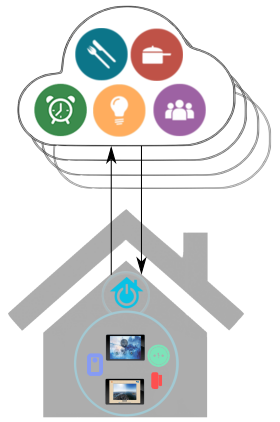
\includegraphics[width=\linewidth,totalheight=\textheight,keepaspectratio]{gfx/archi_domassist}
\caption{Illustration de l'architecture de la plate-forme DomAssist.}
\label{fig:archidomasssit}
\end{marginfigure} 

Dans l'étude DomAssist, un domicile typique est pourvu de quatre
capteurs de contact (porte d'entrée, frigidaire, armoire, \etc), six
détecteurs de mouvements (zone de l'entrée, cuisine, salle de bain,
\etc), et deux capteurs de consommation électrique, qui peuvent
également allumer et éteindre les appareils qui y sont branchés
(chemin lumineux, micro-onde, machine à café, \etc). Le nombre et le
type de capteurs/actionneurs peut varier en fonction de la
configuration du domicile et des activités à surveiller. Enfin, le
domicile est équipé avec deux tablettes. La première, une tablette
fixe, est placée à un endroit central dans le domicile et est toujours
alimentée électriquement. Cette tablette est dédiée aux interactions
de la plate-forme avec l'utilisateur via les notifications émises par
les applications d'assistance, qui alertent l'utilisateur d'une
situation donnée (\eg porte d'entrée ouverte et non surveillée depuis
un certain temps)~\paulcite{consel2015unifying}.  La seconde tablette,
dont la mobilité est autorisée, est utilisée pour les activités
sociales. Elle dispose notamment d'une application de gestion
simplifiée du courrier électronique, avec synthèse vocale. D'autres
applications de communication et des jeux collaboratifs sont également installées.
La Figure~\ref{fig:mapdeployed} montre un exemple de domicile équipé.

\begin{figure*}[]
  \centering
      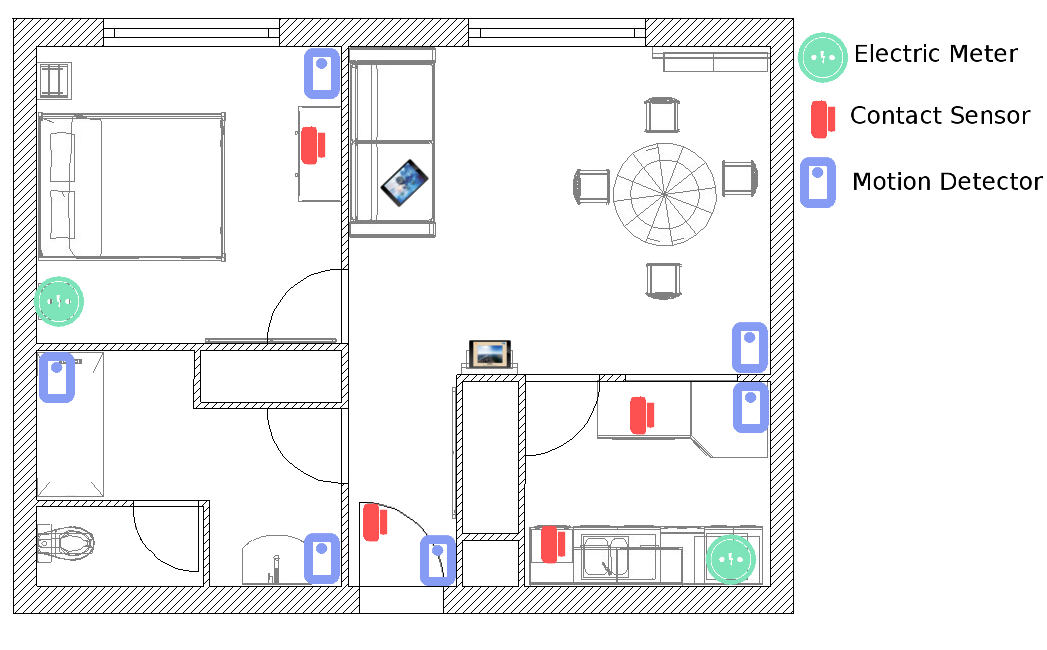
\includegraphics[width=\linewidth,totalheight=\textheight,keepaspectratio]{gfx/Map.png}
      \caption{Exemple de domicile déployé avec son installation de capteurs.}
      \label{fig:mapdeployed}
\end{figure*}


%**********************************************
\section{Scénarios pour le maintien à domicile}\label{domain:scenario}
Les services proposés par les applications disponibles sur la
plate-forme DomAssist concernent l'assistance domiciliaire. Cependant,
il existe de nombreux autres services nécessaires au fonctionnement de
la plate-forme, notamment sa maintenance (\eg infrastructure de
capteurs, infrastructure logicielle, réseau, \etc), qui vont
influencer le bon fonctionnement des services d'assistance.  Ces
services {\em annexes} sont instanciés, non pas directement au sein de
la plate-forme DomAssist en tant qu'applications disponibles, mais avec différents framework spécialisés
(\eg surveillance de la communication réseaux, charge des serveurs,
état des batteries des capteurs, état de l'infrastructure de capteurs,
\etc).

Pour définir quels sont les besoins des intervenants en matière de
services, nous avons recours à la plate-forme d'assistance déployée à
large échelle, aux intervenants ayant contribué à la définition de
services d'assistance, et aux intervenants participant à son
exploitation.  À partir de cet ensemble d'expertise, nous décrivons
dans la Table~\ref{scenario-fig}, quelques scénarios illustrant la
variété d'intervenants et la variété de préoccupations nécessaires au maintien à
domicile de personnes âgées, lorsque des services d'assistance sont
sensibles au contexte.


\begin{table*}[!h]
\begin{small}
\begin{tabular}{| p{2cm} | l | p{2.3cm} | p{7.5cm} |} \hline
{\bf Stakeholder} & {\bf Domain} & {\bf Name} & {\bf Description} \\ \hline \hline
Older adult& Safety & Door Alert & Entrance door \uline{is open} and  \uline{is unattended} \dotuline{for 5 minutes} \\ \hline
Caregiver & Daily Activities 
       & Reheating  A Frozen Meal 
          & Freezer \dashuline{gets used} and stove \dashuline{gets turned on} \dotuline{within 10 minutes} or Freezer \dashuline{gets used} during stove \uline{is on},
during \uline{lunch time} (or dinner time) \\ \hline
 Home Technician
               & Maintenance & Presence Dependency 
                  & The cupboard \dashuline{gets opened} in the kitchen, while a presence in the kitchen \uline{is false} \\ \hline
Home Technician
   & Maintenance 
        & Communication Failure 
             & A sensor \uline{fails to communicate} \dotuline{for 24 hours} %and its status does not \dashuline{get updated} 
\\ \hline
\end{tabular}
\end{small}
\vspace{5mm}
\label{scenario-fig}
\caption{Example de scénarios de services d'assistance.}
\end{table*}

Le premier scénario concerne la sécurité de l'utilisateur. Ce scénario
surveille la porte d'entrée pour s'assurer qu'elle ne reste pas
ouverte trop longtemps sans être surveillée.  Le deuxième scénario
implique à la fois l'utilisateur et l'aidant. Il illustre un besoin
exprimé par les aidants, en fournissant un service qui rappelle à
l'utilisateur une routine du quotidien, dans le cas où il ne l'aurait
pas réalisée (dans l'exemple, la préparation du repas). La formulation du
scénario est déterminée par l'utilisateur qui va définir lui-même la
façon dont il effectue ses routines quotidiennes.
Les deux derniers scénarios concernent des besoins exprimés par les techniciens 
pour garder opérationnels les domiciles sensible au contexte. 
Le premier scénario de maintenance détecte l'utilisation d'un placard sans que 
celle-ci soit recouverte par la détection d'une présence. 
Le second scénario de maintenance détecte quand la passerelle échoue à 
communiquer avec un capteur~;
cette situation se produit lorsque le capteur n'a plus de batterie ou dysfonctionne.

Ces scénarios offrent un aperçu des types de services sensibles au contexte 
nécessaires pour le maintien à domicile de personnes âgées. 
Ces services fournissent directement une assistance ou servent de support au 
bon fonctionnement de la plate-forme.
Certains services tels que ``Door Alert'', peuvent convenir à la plupart des 
utilisateurs. En revanche, d'autres services, typiquement les services concernant 
les activités du quotidien, nécessitent un certain degré de personnalisation pour 
être efficaces. Ceci est illustré par l'activité de préparation de repas et 
le scénario ``Reheating a Frozen Meal''.

De même, ``Communication Failure'' peut s'appliquer à n'importe quel 
domicile sensible au contexte, alors que ``Presence Dependency'' demande 
d'instancier les règles en fonction de la localisation des capteurs. 

Il est à noter que la formulation de certains scénarios, principalement les scénarios de sécurité de la personne ou les scénarios de maintenance, décrit des situations anormales. Par exemple, pour le scénario de ``Presence Dependency'', la situation normale serait décrite ainsi~: {\it ``Quand le placard est est ouvert dans la cuisine, la présence dans la cuisine est vraie''}. Or, dans ces cas là, le but de ces scénarios est d'identifier les situations inhabituelles, c'est donc ces situations qu'ils doivent décrire.

Une autre observation frappante est que certains services de maintenance reprennent directement des règles
qui faisaient partie du modèle d'infrastructure des capteurs, décrit dans le Chapitre~\ref{cha:fiabilite},
sauf qu'elles sont maintenant formulées par la négative, pour chercher les situations non-désirées,
comme expliqué ci-haut. En fait, {\em toutes} les régles du modèle explicite d'infrastructure peuvent
être ainsi exprimées comme des services d'acquisition de contexte, où le contexte concerne alors
les dysfonctionnements de l'infrastructure. Ainsi, le spectre des services contextuels dans une
maison connectée inclut comme un sous-ensemble le modèle d'infrastructure, dans le spectre bien plus large 
des services destinés à tous les intervenants de l'assistance domiciliaire.

\section{Analyse de commonalités et variabilités}\label{domain:commonvar}
Les scénarios définis nous permettent de faire une étude de commonalités et de variabilités.

\subsection{Commonalités} 
Tous les services se réfèrent à une notion d'{\em environnement} dans 
lequel sont effectuées les mesures. Ces mesures observent des interactions 
qui peuvent se passer soit dans l'environnement physique (\eg un mouvement détecté), soit dans 
l'environnement numérique (\eg un rappel d'évènement délivré par un agenda). 
Concernant ces mesures de l'environnement, nous avons identifiés deux concepts 
récurrents dans les scénarios étudiés~: les évènements et les états.
Un {\em évènement} définit une mesure de l'environnement au moment où 
l'interaction correspondante se produit (\eg une porte {\em devient} ouverte/fermée) -- les 
évènements sont soulignés avec des pointillés dans les scénarios de la Table\ref{scenario-fig}.
Un {\em état} exprime l'accès au statut courant d'une mesure préalable de l'environnement
%la persistance d'un évènement dans le temps 
(\eg la porte 
{\em est} ouverte/fermée) -- les états soulignés avec une ligne pleine dans 
la Table~\ref{scenario-fig}.
Ces deux concepts d'état et d'évènement permettent donc d'exprimer 
soit le moment où une interaction se produit, pour les évènements, soit
le statut d'une interaction déjà produite qui persiste dans 
le temps, pour les états.

Il est possible également d'identifier dans les scénarios, des concepts de 
{\em composition}. Spécifiquement, la combinaison de mesures d'environnement 
peut définir un {\em ordre} dans lequel les interactions doivent arriver et 
la {\em durée}, tant des interactions que des compositions -- ces contraintes 
sont soulignées avec des points dans la 
Table~\ref{scenario-fig}.

\subsection{Variabilités} 
Les mesures environnementales peuvent être réalisées 
par une variété d'entités, matérielles (\eg capteurs), logicielles (\eg agenda), 
locales (\eg porte), distante (\eg nouvel email), \etc 
Le niveau d'abstraction varie énormément selon les mesures environnementales. 
Par exemple, un évènement peut être produit par un capteur, sitôt qu'un 
mouvement est détecté dans l'entrée. Parallèlement, cette même interaction 
peut servir pour être agrégée avec d'autres évènements et produire un évènement
``rentrée au domicile''. 
Plusieurs contraintes d'ordre sont possibles pour la composition des 
interactions. Une interaction peut en {\em précéder} une autre, une interaction 
peut se produire {\em durant} une autre, et une interaction peut en {\em chevaucher} une 
autre. Cependant, toutes ces contraintes ne sont pas applicables à tous les types 
d'interactions (\ie évènements et états). Par exemple, seulement deux états 
peuvent se chevaucher, alors que les évènements ne peuvent pas se
chevaucher à cause de leur nature ponctuelle.
% dans la pratique cette situation suppose deux interactions strictement simultanées.

\subsection{Concepts spécifiques au domaine}
%Reccurrence dans les séquences à detecter

Suivant cette analyse, nous pouvons d'ores et déjà exprimer certains
concepts.  Nous retrouvons un modèle d'environnement, comme évoqué en
Section~\ref{seq:fiabilite:cas}, avec des informations sur
l'interaction (le type d'interaction mesurée, sa localisation,
la valeur mesurée, la positionnement dans le temps) et les niveaux
d'abstraction d'une interaction (\eg physiques, logiciels, \etc).
%(\eg état du capteur, type d'interaction mesurée, localisation de l'interaction, timer, agenda, etc).
Il est maintenant possible de définir plus précisément le concept d'évènement et d'état~:

\myparagraph{Évènement~:} un changement de valeur, pour une entité mesurée, qui se produit à un moment donné. 

\myparagraph{État~:} Une valeur qui subsiste pendant une période. L'état débute à un moment donné et finit à un autre moment.

Pour composer ces états et évènement dans le temps, nous avons extrait de notre analyse des opérateurs de composition (\eg précédence, chevauchement, \etc).

\section{Besoins communs}\label{domain:needs}
L'analyse des services d'une plate-forme d'assistance domiciliaire met en évidence certaines contraintes indispensables à l'exploitation des services. Du fait de leur sensibilité au contexte, et leur objectifs parfois critiques dans l'assistance domiciliaire (\eg sécurité, maintenance, \etc), les services doivent être capables de réagir rapidement aux mesures d'environnement qu'ils traitent.

De plus, des services avec des objectifs différents doivent pouvoir accéder aux mêmes données pour effectuer des traitements différents.
La variété d'intervenants et la variété de leur expertise impliquent une forte hétérogénéité de données qu'il faut exprimer en terme d'état et d'évènements.

Les services expriment un ensemble d'interactions qui peut revenir de façon récurrente dans le flux d'évènements d'interactions. Par exemple, les évènements décrivant l'activité de préparation d'un repas reviennent typiquement tous les jours. Par conséquent, un service vérifiant que l'activité à été effectué doit être testé de manière récurrente.

Comme observé, il y a une forte composante temporelle dans l'expression des services. Tant pour expliciter la durée de la persistance d'un état, que pour exprimer de simples relations entre états/évènements et la durée de cette relation, cette composante temporelle doit être partie intégrante de l'expressivité des services sensibles au contexte.

La variété d'intervenants implique également autant de manières de formuler un scénario de service.
Les scénarios exprimés par les intervenants doivent couvrir l'ensemble des services nécessaires à une plate-forme d'assistance de maintien à domicile des personnes âgées. Il faut donc être capable de proposer une solution permettant d'exprimer ces services en couvrant leur spectre d'expertise et d'objectifs. Cependant, malgré l'hétérogénéité des données captées et malgré la large variété des besoins entre les intervenants des différents domaines d'expertise, ces services sensibles au contextes agencent des concepts communs qui permettent d'uniformiser leur formulation et leur traitements.
